\documentclass[aspectratio=169,t]{beamer}

\usepackage[utf8]{inputenc}
\usepackage{amsmath}

\usepackage{multicol}
\usepackage{multirow}
\usepackage{textcomp} % to use \textmu
\usepackage[absolute,overlay]{textpos} % to place floating text boxes with \begin{textblock*}{width}(x,y)
\usepackage{tcolorbox}

\usepackage{tikz}
\usetikzlibrary{decorations.pathreplacing}

\usepackage{graphicx}
\graphicspath{{./figuras/}}

\setbeamertemplate{navigation symbols}{}

\title{Clase 29}
\subtitle{Aplicaciones digitales del MOSFET}
\author{Dr.-Ing. Juan José Montero-Rodríguez}
\institute{Escuela de Ingeniería Electrónica}
\date{Semestre II-2023}
\titlegraphic{\includegraphics[height=8mm]{logoTEC.png}}


\begin{document}

\begin{frame}
\titlepage
\end{frame}


\section{Interruptor}
\begin{frame}{MOSFET como Interruptor Serie}
\centering
\includegraphics[width=10cm]{MOSserie1}

$I_D = K/2 (V_{DD} - v_o - V_{TH})^2$, $V_{TH}$ incluyendo efecto de substrato

\vspace{5mm}
\includegraphics[width=10cm]{MOSserie2}

$I_D = K/2 (V_{DD} - V_{TH0})^2$, $V_{TH0}$ no incluye efecto de substrato
\end{frame}


\begin{frame}{Limitaciones del MOSFET como interruptor}

\vspace{-5mm}
\begin{columns}

\begin{column}{0.4\textwidth}

\begin{figure}
    \centering
    \includegraphics[width=\textwidth]{figuras/passgate_capacitances.png}
\end{figure}

\end{column}

\begin{column}{0.6\textwidth}

\[ t_{delay} = 0.7 \cdot R_n C_{tot} = 0.7 \cdot R_n \cdot \left( C_L + \dfrac{C_{ox}}{2} \right) \]

\end{column}
    
\end{columns}

\begin{figure}
    \centering
    \includegraphics[width=0.85\textwidth]{figuras/passgate_response.png}
\end{figure}


\end{frame}



\begin{frame}{Compuerta de transmisión}

La compuerta de transmisión es un interruptor que funciona en ambas direcciones:

\begin{columns}

\begin{column}{0.3\textwidth}

\begin{figure}
    \centering
    \includegraphics[width=0.8\textwidth]{figuras/transmission_gate_1.png}
\end{figure}

\begin{figure}
    \centering
    \includegraphics[width=0.8\textwidth]{figuras/transmission_gate_2.png}
\end{figure}

\end{column}

\begin{column}{0.7\textwidth}

\begin{figure}
    \centering
    \includegraphics[width=\textwidth]{figuras/transmission_gate_3.png}
\end{figure}

\end{column}
    
\end{columns}

\end{frame}


\section{Inversor}
\begin{frame}{Inversor CMOS}
\centering
CMOS: Complementary Metal Oxide Semiconductor (1963)

Circuitos con transistores PMOS y NMOS

\begin{columns}
\begin{column}{10cm}
\includegraphics[width=10cm]{inverter1}
\end{column}
\begin{column}{4cm}
\includegraphics[width=4cm]{inverter2}
\end{column}
\end{columns}


$V_in > V_{THN}$ , $V_{in} = V_{DD}$ $\Rightarrow$ NMOS activado, PMOS inactivo

$\Rightarrow$ $V_{out} = 0 V$: NMOS en región lineal, PMOS en región de corte
\end{frame}


\begin{frame}{Inversor CMOS}
\includegraphics[width=10cm]{inverter1}

\begin{textblock*}{4cm}(11cm,1cm)
	\includegraphics[width=4cm]{inverter2}
\end{textblock*}

\begin{columns}
\begin{column}{0.7\textwidth}
$ V_{DD} - V_{in} > |V_{THP}|$ , $V_{in} = 0 V$ $\Rightarrow$ PMOS activo, NMOS inactivo

$\Rightarrow V_{out} = V_{DD}$: PMOS en región lineal, NMOS en región de corte

\vspace{2mm}
Ambos transistores activos durante transiciones de $v_{in}$ $\Rightarrow$ corto circuito temporal de VDD a tierra $\Rightarrow$ consumo de potencia
\end{column}
\begin{column}{0.3\textwidth}
\end{column}
\end{columns}

\vspace{2mm}
\begin{columns}
\begin{column}{0.3\textwidth}
	\centering Potencia consumida
	
	debido a carga
	
	capacitiva
\end{column}
\begin{column}{0.3\textwidth}
	\[ P = C_{load} \cdot f \cdot {V_{DD}}^2 \]
\end{column}
\begin{column}{0.4\textwidth}
	C\textsubscript{L}: capacitancia de carga
	
	V\textsubscript{DD}: voltaje de alimentación
	
	f: frecuencia de conmutación
\end{column}
\end{columns}

\end{frame}


\begin{frame}{Curva de transferencia del inversor CMOS}

La curva de transferencia se mide variando la entrada, y midiendo la tensión de salida.

\begin{figure}
    \centering
    \includegraphics[width=0.8\textwidth]{figuras/inverter_transfer_1.png}
\end{figure}



\end{frame}


\begin{frame}{Punto de disparo del inversor CMOS}

\begin{columns}

\begin{column}{0.5\textwidth}

\begin{figure}
    \centering
    \includegraphics[width=\textwidth]{figuras/inverter_transfer_2.png}
\end{figure}

\end{column}

\begin{column}{0.5\textwidth}

\[ V_{SP} = \dfrac{\sqrt{\dfrac{\beta_n}{\beta_p}} \cdot V_{THn} + (V_{DD} - V_{THp})}{1 + \sqrt{\dfrac{\beta_n}{\beta_p}}} \]
\[ \beta_n = \mu_n C_{ox}' \dfrac{W}{L} \]
\[ \beta_p = \mu_p C_{ox}' \dfrac{W}{L} \]

\end{column}

\end{columns}

\end{frame}


\begin{frame}{Inversor de tres estados}

Se conecta una compuerta de transmisión a la salida de un inversor CMOS:

\begin{columns}

\begin{column}{0.5\textwidth}

\begin{figure}
    \centering
    \includegraphics[width=0.7\textwidth]{figuras/three_state_inverter.png}
\end{figure}

\end{column}

\begin{column}{0.5\textwidth}

\begin{table}[H]
    \centering
    \begin{tabular}{|p{1cm}|p{1cm}|p{1cm}|}
        \hline \textbf{S}  & \textbf{In}   & \textbf{Out}  \\
        \hline 0           & 0             & Z             \\
        \hline 0           & 1             & Z             \\
        \hline 1           & 0             & 1             \\
        \hline 1           & 1             & 0             \\
        \hline 
    \end{tabular}
\end{table}

\end{column}

\end{columns}

\end{frame}


\section{Compuertas}
\begin{frame}{Compuerta NAND}
\centering
\includegraphics[width=10cm]{gate-NAND}

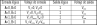
\includegraphics[width=11cm]{tabla-NAND}
\end{frame}


\begin{frame}{Compuerta NOR}
\centering
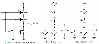
\includegraphics[width=10cm]{gate-NOR}

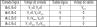
\includegraphics[width=11cm]{tabla-NOR}
\end{frame}


\begin{frame}{NAND de tres entradas}

\begin{columns}

\begin{column}{0.5\textwidth}

\begin{figure}
    \centering
    \includegraphics[width=0.7\textwidth]{figuras/aoi_nand_1.png}
\end{figure}

\end{column}

\begin{column}{0.5\textwidth}

\begin{figure}
    \centering
    \includegraphics[width=0.7\textwidth]{figuras/aoi_nand_2.png}
\end{figure}

\end{column}

\end{columns}
    
\end{frame}


\begin{frame}{NOR de tres entradas}

\begin{columns}

\begin{column}{0.5\textwidth}

\begin{figure}
    \centering
    \includegraphics[width=0.7\textwidth]{figuras/aoi_nor_1.png}
\end{figure}

\end{column}

\begin{column}{0.5\textwidth}

\begin{figure}
    \centering
    \includegraphics[width=0.7\textwidth]{figuras/aoi_nor_2.png}
\end{figure}

\end{column}

\end{columns}
    
\end{frame}




\section{Memorias}
\begin{frame}{Estructura de memorias RAM}

\begin{figure}[H]
    \centering
    \includegraphics[width=0.7\textwidth]{figuras/estructura_memorias_ram.png}
\end{figure}
    
\end{frame}


\begin{frame}{Celdas de memoria SRAM}
\begin{itemize}
	\item Las memorias RAM son volátiles = pierden los datos al remover la alimentación
	\item SRAM: Static Random Access Memory
	\item Dato se guarda con cerrojo de dos inversores cross-coupled por celda
	\item Los transistores de línea de palabra conectan el cerrojo con los circuitos de lectura y escritura
\end{itemize}

\centering
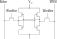
\includegraphics[width=7cm]{SRAM}
\end{frame}


\begin{frame}{Celdas de memoria DRAM}
\begin{itemize}
	\item DRAM: Dynamic Random Access Memory
	\item Dato se guarda en un capacitor de almacenamiento: capacitor cargado = '1', descargado ='0'
	\item El transistor de línea de palabra connecta el capacitor de almacenamiento con el circuito de lectura/escritura
	\item Corriente de fuga descarga capacitor $\Rightarrow$ dato debe reescribirse periódicamente = refrescamiento de datos
\end{itemize}

\centering
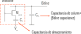
\includegraphics[width=10cm]{DRAM}
\end{frame}





\begin{frame}{La celda de memoria de compuerta flotante}

En esta estructura, el poly1 está flotando.

\begin{columns}

\begin{column}{0.5\textwidth}

\begin{figure}
    \centering
    \includegraphics[width=\textwidth]{figuras/floating_gate_1.png}
\end{figure}

\end{column}

\begin{column}{0.5\textwidth}

\begin{figure}
    \centering
    \includegraphics[width=\textwidth]{figuras/floating_gate_2.png}
\end{figure}

\end{column}

\end{columns}

\vspace{5mm}
Al acumular carga en la compuerta, cambia la tensión $V_{TH}$.

\begin{figure}
    \centering
    \includegraphics[width=0.4\textwidth]{figuras/floating_gate_3.png}
\end{figure}

\end{frame}


\begin{frame}{Memorias EEPROM}

En las memorias EPROM, la carga se coloca por el método de  inyección de portadores calientes desde el canal.

\begin{figure}
    \centering
    \includegraphics[width=0.5\textwidth]{figuras/eeprom.png}
\end{figure}

\begin{itemize}
    \item La tensión $V_{DDP}$ que  se requiere para lograr  programar la memoria es alta ($\approx 25\ V$).
    \item Los electrones pueden superar la barrera de potencial del SiO\textsubscript{2}.
    \item La memoria se borra con luz UV.
    \item La luz aumenta la conductividad del SiO\textsubscript{2} (liberando la carga).
\end{itemize}

\end{frame}


\begin{frame}{Memorias flash}

Para programarla se utiliza efecto túnel (Fowler-Nordheim).

\begin{columns}

\begin{column}{0.5\textwidth}

\centering
\textbf{Escritura}

\begin{figure}[H]
    \centering
    \includegraphics[width=0.9\textwidth]{figuras/flash_1.png}
\end{figure}

\end{column}

\begin{column}{0.5\textwidth}

\centering
\textbf{Borrado}

\begin{figure}[H]
    \centering
    \includegraphics[width=0.9\textwidth]{figuras/flash_2.png}
\end{figure}

\end{column}

\end{columns}

\vspace{5mm}
\begin{itemize}
    \item \textbf{Leer} la memoria no genera problemas. Para leer la memoria se debe ``medir" la tensión de umbral. Esto no requiere modificar la carga existente en el poly1.
    \item \textbf{Escribir} o \textbf{borrar} la memoria desgasta el óxido, debido a las altas  tensiones de programación. Memorias NAND Flash SLC soportan $\sim$100000 ciclos. Memorias 3D-NAND Flash TLC soportan $\sim$1000-3000 ciclos.
\end{itemize}
    
\end{frame}


\section{Potencia}
\begin{frame}{Consumo de Potencia}
\centering
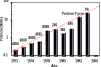
\includegraphics[width=12cm]{power}

\raggedright
En general, en los circuitos integrados,

Disipación por carga capacitiva $>>$ Potencia corto circuito $>>$ Potencia estática
\end{frame}


\begin{frame}{Potencia Estática}
\centering
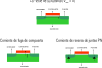
\includegraphics[width=11cm]{pstatic}
\end{frame}


\begin{frame}{Potencia Dinámica}
\begin{itemize}
	\item Potencia dinámica debido a corriente de corto circuito
\end{itemize}

\begin{columns}

	\begin{column}{0.5\textwidth}
 
		\centering
		\includegraphics[width=5cm]{pdynamic}
  
	\end{column}
 
	\begin{column}{0.5\textwidth}
 
		Para V\textsubscript{IN}=V\textsubscript{OUT} ambos transistores operan en saturación
		
		$\Rightarrow$ ambos transistores conducen, permitiendo un flujo de corriente de VDD a tierra
		
		\textcolor{red}{$\Rightarrow$ Corriente de corto circuito}
		
		\vspace{3mm}
		Potencia disipada:
		%
		\[ P_{SC} = I_{SC} \cdot V_{DD} = \dfrac{2}{3} \cdot K \cdot \dfrac{t_r}{T} \left(\dfrac{V_{DD}}{2} - V_{TH}\right)^3 \]
		%
		t\textsubscript{r}: tiempo de subida (se asume t\textsubscript{r} = t\textsubscript{f})
		
		T: período de V\textsubscript{IN}
  
	\end{column}
 
\end{columns}

\end{frame}


\begin{frame}{Potencia Dinámica}
\begin{itemize}
	\item Potencia dinámica debido a cargas capacitivas
\end{itemize}

\begin{columns}

	\begin{column}{0.5\textwidth}
 
		\centering
		\includegraphics[width=5cm]{pdynamic2}
  
	\end{column}
 
	\begin{column}{0.5\textwidth}
 
		Capacitancia de carga debido a:
		
		-C\textsubscript{OX} de compuertas siguientes
		
		-C\textsubscript{OX} propia
		
		-C\textsubscript{W}, capacitancia parásita de interconexión
		
		Representadas por C\textsubscript{L}
		
		\vspace{3mm}
		Potencia disipada:
		%
		\[ P_L = A \cdot f \cdot C_L \cdot {V_{DD}}^2 \]
		%
		f : frecuencia de conmutación
		
		C\textsubscript{L}: capacitancia de carga
		
		A: factor de actividad = probabilidad de conmutación
  
	\end{column}
 
\end{columns}

\end{frame}


\section{Referencias}
\begin{frame}{Lecturas recomendadas}

\begin{itemize}
    \item Baker, R. J. (2010). CMOS: Circuit Design, Layout and Simulation, 3rd edition, IEEE Series on Microelectronic Systems, pp. 321-374. Wiley, New Jersey, United States.
    \item Baker, R. J. CMOSedu.com, en línea: \url{http://cmosedu.com/}
    \item Razavi, B. (2013). Fundamentals of Microelectronics, 2nd edition. Chapter 16: Digital CMOS Circuits, pp. 760-800, Wiley, Los Angeles, California.
\end{itemize}

\end{frame}


\end{document}
